% ============================================================
%  Sanity — Guide d'utilisation (pour les clients)
%  Compiler :  pdflatex guide-sanity.tex   (deux fois, pour la table des matières)
%  Les captures d'écran sont dans ./images/
%  Personnaliser : les quatre commandes \Editeur, \Support... ci-dessous.
% ============================================================
\documentclass[11pt,a4paper]{report}

% ---------- personnalisation
\newcommand{\Editeur}{Votre société}                 % qui édite / installe Sanity
\newcommand{\SupportMail}{support@votre-societe.ma}
\newcommand{\SupportTel}{+212 5 22 00 00 00}
\newcommand{\VersionGuide}{Version 1.0 — octobre 2026}

% ---------- paquets
\usepackage[T1]{fontenc}
\usepackage[utf8]{inputenc}
\usepackage[french]{babel}
\usepackage{lmodern}
\usepackage{microtype}
\usepackage[a4paper,margin=2.2cm,headheight=14pt]{geometry}
\usepackage{graphicx}
\usepackage[table]{xcolor}
\usepackage{tcolorbox}
\tcbuselibrary{skins,breakable}
\usepackage{enumitem}
\usepackage{titlesec}
\usepackage{fancyhdr}
\usepackage{booktabs}
\usepackage{tabularx}
\usepackage{array}
\usepackage[hidelinks]{hyperref}
\usepackage{bookmark}

% ---------- couleurs (palette Sanity)
\definecolor{sbleu}{HTML}{2A78D6}
\definecolor{sbleufonce}{HTML}{184F95}
\definecolor{sorange}{HTML}{EB6834}
\definecolor{svert}{HTML}{0CA30C}
\definecolor{sjaune}{HTML}{FAB219}
\definecolor{srouge}{HTML}{D03B3B}
\definecolor{sgris}{HTML}{52514E}
\definecolor{sfond}{HTML}{F4F6FA}

\hypersetup{pdftitle={Sanity — Guide d'utilisation}, pdfauthor={\Editeur}}

% ---------- mise en page
\setlength{\parindent}{0pt}
\setlength{\parskip}{6pt}
\setlist{itemsep=2pt,topsep=4pt}
\titleformat{\chapter}[display]{\normalfont\bfseries\color{sbleufonce}}{\large\scshape Chapitre \thechapter}{4pt}{\Huge}
\titlespacing*{\chapter}{0pt}{-10pt}{18pt}
\titleformat{\section}{\normalfont\Large\bfseries\color{sbleu}}{\thesection}{0.8em}{}
\titleformat{\subsection}{\normalfont\large\bfseries\color{sbleufonce}}{\thesubsection}{0.8em}{}
\pagestyle{fancy}
\fancyhf{}
\fancyhead[L]{\small\color{sgris}Sanity — Guide d'utilisation}
\fancyhead[R]{\small\color{sgris}\leftmark}
\fancyfoot[L]{\small\color{sgris}\Editeur}
\fancyfoot[R]{\small\color{sgris}\thepage}
\renewcommand{\headrulewidth}{0.3pt}
\renewcommand{\chaptermark}[1]{\markboth{#1}{}}
\fancypagestyle{plain}{\fancyhf{}\fancyfoot[R]{\small\color{sgris}\thepage}\renewcommand{\headrulewidth}{0pt}}

% ---------- commandes du guide
% Chemin de menu :  \menu{Stock › Articles}
\newcommand{\menu}[1]{\tcbox[on line, colback=sfond, colframe=sbleu!40, boxrule=0.4pt, arc=2pt, left=3pt, right=3pt, top=1pt, bottom=1pt]{\small\sffamily #1}}
% Bouton à l'écran :  \bouton{Nouvel article}
\newcommand{\bouton}[1]{\tcbox[on line, colback=sbleu, colupper=white, boxrule=0pt, arc=3pt, left=4pt, right=4pt, top=1pt, bottom=1pt]{\small\sffamily\bfseries #1}}
% Champ / libellé
\newcommand{\champ}[1]{\textsf{\textbf{#1}}}

\newtcolorbox{astuce}{enhanced, breakable, colback=svert!6, colframe=svert, boxrule=0pt, leftrule=3pt, arc=2pt, title={\textbf{Astuce}}, coltitle=svert!70!black, attach title to upper={\ \ }, fonttitle=\sffamily}
\newtcolorbox{attention}{enhanced, breakable, colback=sjaune!10, colframe=sjaune, boxrule=0pt, leftrule=3pt, arc=2pt, title={\textbf{Attention}}, coltitle=sjaune!50!black, attach title to upper={\ \ }, fonttitle=\sffamily}
\newtcolorbox{droit}{enhanced, breakable, colback=sbleu!6, colframe=sbleu, boxrule=0pt, leftrule=3pt, arc=2pt, title={\textbf{Droit nécessaire}}, coltitle=sbleufonce, attach title to upper={\ \ }, fonttitle=\sffamily}

% Capture d'écran :  \capture{fichier}{légende}{largeur}
\newcommand{\capture}[3]{%
  \begin{figure}[htbp]\centering
  \fcolorbox{sbleu!25}{white}{\includegraphics[width=#3\linewidth]{images/#1}}
  \caption{#2}\end{figure}}

% Étapes numérotées
\newcommand{\pastille}[1]{\tcbox[on line, colback=sbleu, colupper=white, boxrule=0pt, arc=6pt, left=2pt, right=2pt, top=0pt, bottom=0pt]{\footnotesize\bfseries #1}}
\newenvironment{etapes}{\begin{enumerate}[label={\protect\pastille{\arabic*}}, leftmargin=2em, itemsep=4pt]}{\end{enumerate}}

\begin{document}

% ============================================================ couverture
\begin{titlepage}
  \thispagestyle{empty}
  \begin{tcolorbox}[enhanced, colback=sbleufonce, colframe=sbleufonce, arc=0pt, boxrule=0pt, left=24pt, right=24pt, top=36pt, bottom=36pt, width=\linewidth]
    \color{white}
    {\sffamily\small PLATEFORME DE NÉGOCE}\par\vspace{6pt}
    {\sffamily\bfseries\fontsize{44}{48}\selectfont Sanity}\par\vspace{10pt}
    {\sffamily\LARGE Guide d'utilisation}\par\vspace{18pt}
    {\sffamily\normalsize Stock multi-dépôts · Ventes revendeurs \& installateurs · Comptoir · Livraisons · Commerciaux · Achats · Analyses}
  \end{tcolorbox}
  \vspace{1.2cm}
  \begin{center}
    \fcolorbox{sbleu!25}{white}{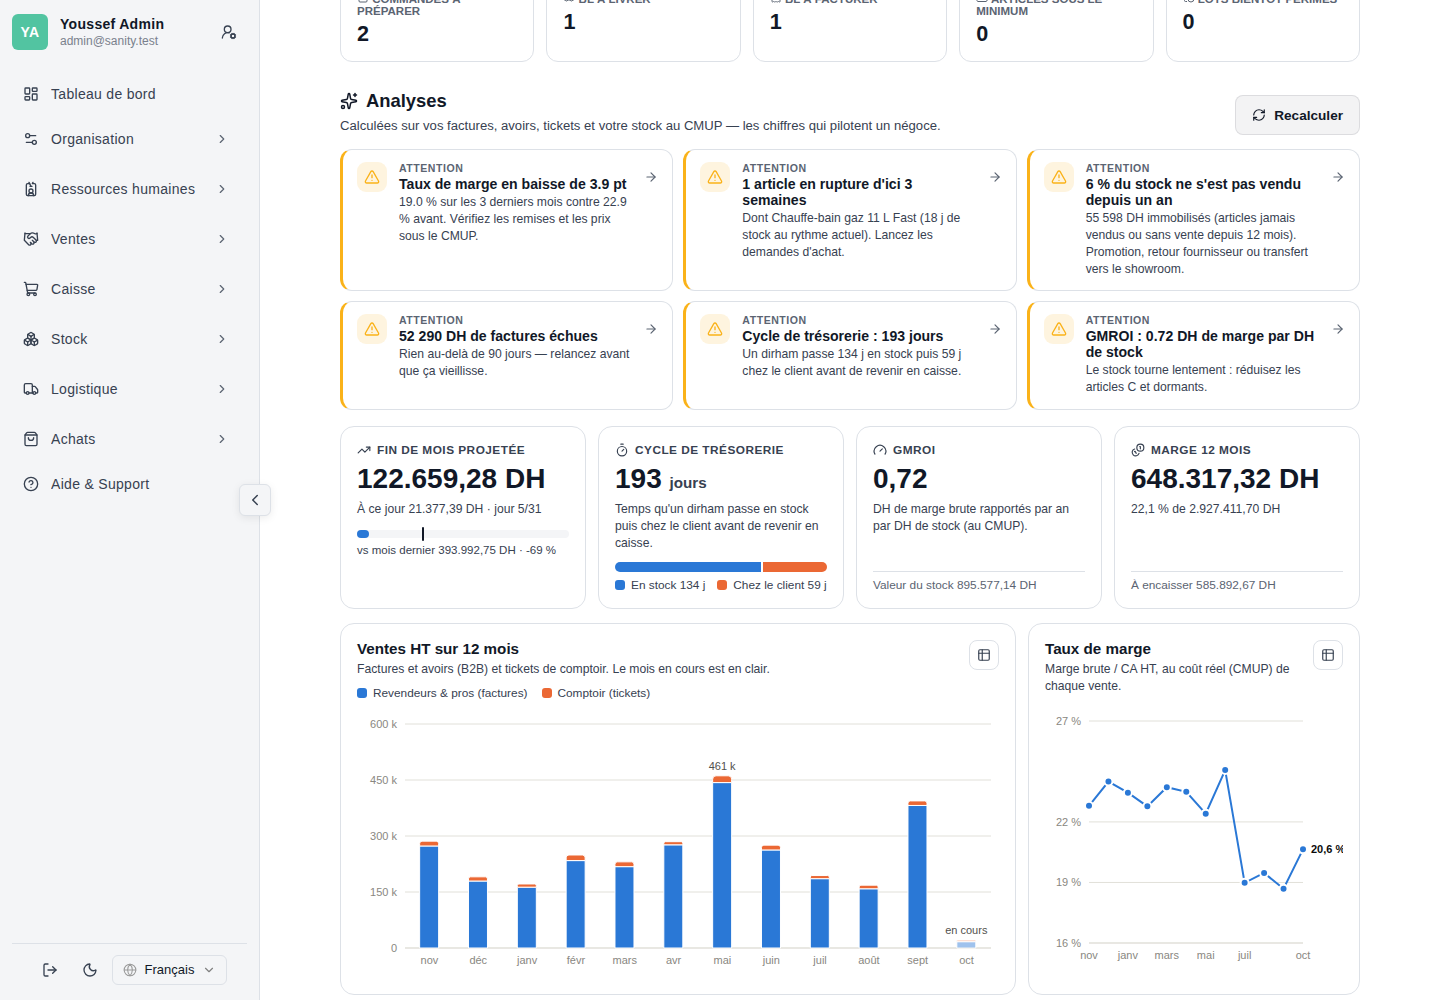
\includegraphics[width=0.86\linewidth]{images/40_analyses_clair_1.png}}
  \end{center}
  \vfill
  {\sffamily\small\color{sgris}
  \begin{tabularx}{\linewidth}{@{}X r@{}}
    \textbf{\Editeur} & \VersionGuide \\
    Assistance : \SupportMail & \SupportTel
  \end{tabularx}}
\end{titlepage}

\tableofcontents
\clearpage

% ============================================================
\chapter{Bienvenue dans Sanity}

Sanity est la plateforme de gestion pensée pour les \textbf{négociants et grossistes} : quincaillerie, sanitaire, électricité, peinture\dots{} Vous achetez à vos fournisseurs, vous stockez dans un ou plusieurs dépôts, et vous revendez à des revendeurs, à des installateurs, à des entreprises du bâtiment et au comptoir. Sanity relie toutes ces étapes : chaque achat met à jour le coût de vos articles, chaque vente sort le stock à son vrai coût, et vos marges, vos créances et votre trésorerie se calculent toutes seules.

\section*{Ce que vous trouverez dans ce guide}
\begin{itemize}
  \item Les premiers pas : se connecter, se repérer, choisir sa langue et son thème.
  \item Le tableau de bord et ses \textbf{analyses} : ce que signifient les chiffres et comment agir.
  \item Le \textbf{stock} : articles, photos, prix, dépôts, transferts, inventaires.
  \item Les \textbf{ventes} : clients, tarifs, devis, commandes, bons de livraison, factures, encaissements, recouvrement.
  \item La \textbf{caisse} (comptoir / showroom), les \textbf{livraisons} et les \textbf{achats}.
  \item L'\textbf{assistant} intégré, les droits d'accès et les réponses aux questions fréquentes.
\end{itemize}

\begin{astuce}
À tout moment, cliquez sur le bouton \bouton{Assistant} en bas à droite de l'écran et posez votre question en français (\og Comment faire un transfert entre dépôts ? \fg). Il vous répond avec le menu et les étapes.
\end{astuce}

% ============================================================
\chapter{Premiers pas}

\section{Se connecter}
\begin{etapes}
  \item Ouvrez l'adresse de votre plateforme Sanity dans votre navigateur (Chrome, Edge, Firefox ou Safari récents).
  \item Saisissez votre adresse e-mail et votre mot de passe, puis cliquez sur \bouton{Se connecter}.
  \item Si la double authentification est activée sur votre compte, saisissez le code reçu.
\end{etapes}
Vous arrivez sur le \textbf{Tableau de bord}.

\section{Se repérer à l'écran}
\begin{itemize}
  \item \textbf{La barre latérale} (à gauche) contient les menus : Tableau de bord, Organisation, Ressources humaines, Mon espace, Ventes, Caisse, Stock, Logistique, Achats, Aide \& Support. Le bouton \bouton{<} la replie pour gagner de la place.
  \item \textbf{Vous ne voyez que ce qui vous concerne} : les menus et les boutons dépendent des droits de votre compte (voir chapitre~\ref{chap:droits}).
  \item \textbf{En bas de la barre} : déconnexion, thème clair ou sombre (icône soleil / lune), langue (français, anglais, arabe\dots).
  \item \textbf{Plusieurs sociétés} : si votre groupe gère plusieurs sociétés, un sélecteur \champ{Entreprise} en haut des pages choisit celle que vous consultez.
  \item \textbf{La cloche} (en haut à droite) affiche vos notifications : stock bas, factures échues, demandes d'achat, etc.
\end{itemize}

\section{Rechercher}
Toutes les listes se cherchent de la même façon. Tapez :
\begin{itemize}
  \item le \textbf{début d'un mot} du nom : \og chrom \fg{} trouve \og Mitigeur lavabo chromé \fg{} ;
  \item une \textbf{référence}, même partielle : \og GRO-ES \fg{} ;
  \item un \textbf{code-barres} ou simplement \textbf{ses derniers chiffres} : \og 4570 \fg{} ;
  \item la \textbf{référence d'un fournisseur}.
\end{itemize}
Les accents et les majuscules n'ont pas d'importance. La recherche se fait sur le serveur : elle reste instantanée même avec des dizaines de milliers d'articles.

% ============================================================
\chapter{Le tableau de bord}

\capture{01_dashboard.png}{Le tableau de bord : chiffres du jour et du mois, puis ce qui est à traiter.}{0.92}

\section{Les chiffres du jour}
En haut de l'écran : \textbf{ventes du jour} et \textbf{du mois} (hors taxes), \textbf{marge}, ventes au \textbf{comptoir} du jour, montant \textbf{à encaisser} (dont en retard) et \textbf{valeur du stock} au coût moyen.

\section{À traiter}
Cinq compteurs cliquables : commandes à préparer, bons de livraison à livrer, bons de livraison à facturer, articles sous le stock minimum, lots bientôt périmés. Un clic ouvre directement la liste concernée.

\section{Les analyses}
\begin{droit}
La section \textbf{Analyses} n'apparaît qu'aux comptes qui ont le droit \og Voir les montants \fg. Un commercial ne voit que les chiffres de ses propres clients.
\end{droit}

\capture{38_analyses_sombre_1.png}{Les analyses : constats automatiques, indicateurs clés et ventes sur 12 mois (thème sombre).}{0.92}

\subsection{Les constats « À retenir »}
Sanity lit vos chiffres à votre place et affiche, du plus urgent au moins urgent, des constats en langage clair : \og Taux de marge en baisse de 3,9 pt \fg, \og 1 article en rupture d'ici 3 semaines \fg, \og 52 290 DH de factures échues \fg\dots{} Chaque carte porte un niveau (\textcolor{srouge}{\textbf{Urgent}}, \textcolor{sjaune!70!black}{\textbf{Attention}}, \textcolor{svert}{\textbf{Bonne nouvelle}}, \textcolor{sbleu}{\textbf{À savoir}}) et \textbf{mène à l'écran où agir}.

\subsection{Les indicateurs clés}
\begin{description}[leftmargin=0pt, style=nextline]
  \item[Fin de mois projetée] Le chiffre d'affaires que vous ferez ce mois-ci si le rythme actuel se maintient, comparé au mois dernier.
  \item[Cycle de trésorerie] Le nombre de jours qu'un dirham passe \textbf{en stock} (jours de stock) puis \textbf{chez le client} (jours de crédit) avant de revenir en caisse. Plus il est court, moins vous avez besoin de trésorerie. Pour le réduire : moins de stock dormant, des relances plus rapides.
  \item[GMROI] La marge brute que rapporte, sur un an, chaque dirham immobilisé en stock. Un GMROI de 1,5 signifie que 1 DH de stock rapporte 1,5 DH de marge par an.
  \item[Marge 12 mois] La marge brute réalisée sur les douze derniers mois, au coût réel de chaque vente.
\end{description}

\subsection{Les graphiques}
\begin{itemize}
  \item \textbf{Ventes HT sur 12 mois} : en bleu les factures (revendeurs, installateurs, entreprises), en orange le comptoir. Le mois en cours est plus clair.
  \item \textbf{Taux de marge} mois par mois : une baisse signale des remises trop fortes ou des prix d'achat qui ont augmenté sans que les prix de vente suivent.
  \item \textbf{Analyse ABC de la marge} : les articles de \textbf{classe A} font 80~\% de votre marge. Ce sont eux qu'il ne faut \textbf{jamais} laisser en rupture.
  \item \textbf{Familles} : chiffre d'affaires et taux de marge de chaque famille.
  \item \textbf{Âge du stock} : la valeur de votre stock selon la date de dernière vente de chaque article. Le stock \og jamais vendu \fg{} ou vendu il y a plus d'un an immobilise de l'argent.
  \item \textbf{Créances par ancienneté} : ce qui vous est dû, selon le retard.
  \item \textbf{Ruptures prévues} : les articles qui seront vides d'ici trois semaines au rythme des 90 derniers jours, avec la date et la quantité à commander.
  \item \textbf{Commerciaux} : réalisé, projection de fin de mois et objectif de chacun.
\end{itemize}

\capture{41_analyses_clair_2.png}{Analyse ABC, familles, âge du stock, créances et ruptures prévues (thème clair).}{0.92}

\begin{astuce}
Passez la souris sur un graphique pour lire les valeurs. L'icône \og grille \fg{} en haut à droite de chaque graphique affiche les mêmes chiffres en tableau. Le bouton \bouton{Recalculer} met les analyses à jour immédiatement (sinon elles sont recalculées toutes les 5 minutes).
\end{astuce}

% ============================================================
\chapter{Le stock}

\section{Le catalogue d'articles}
\menu{Stock › Articles}

Le catalogue s'ouvre sur vos \textbf{familles} (Sanitaire, Électricité, Peinture, Quincaillerie\dots). Cliquez sur une famille pour voir ses sous-familles et ses articles. Le fil \og Toutes les familles › Sanitaire › Robinetterie \fg{} vous permet de remonter.

\capture{22_catalogue_families.png}{Le catalogue commence par les familles.}{0.9}

Chaque \textbf{carte article} montre la photo, la marque, l'état du stock (\textcolor{svert}{\textbf{En stock}}, \textcolor{sjaune!70!black}{\textbf{Stock bas}}, \textcolor{srouge}{\textbf{Rupture}}), la quantité et le prix public TTC. Le bouton \bouton{Tableau} affiche la même liste en lignes.

\capture{24_catalogue_articles.png}{Les cartes articles d'une sous-famille.}{0.9}

\subsection{Les trois boutons de chaque article}
\begin{description}[leftmargin=0pt, style=nextline]
  \item[Demande d'achat] Indiquez la quantité souhaitée (Sanity propose de remonter jusqu'au stock maximum) et une note ; la demande part au service achats.
  \item[Prix fournisseurs] Le prix d'achat de l'article chez \textbf{tous} vos fournisseurs : prix catalogue, dernière commande, dernier devis. Le meilleur prix est en tête, les autres affichent leur écart en pourcentage.
  \item[Prix de vente] Les prix de chaque niveau (Revendeur, Gros, Détail, Comptoir), hors taxes et TTC, à l'unité et au carton, avec la marge.
\end{description}

\capture{25_catalogue_supplier-prices.png}{Comparer les prix d'achat de tous les fournisseurs.}{0.85}

\begin{droit}
\og Prix fournisseurs \fg{} et les marges sont réservés aux comptes qui voient les montants. \og Demande d'achat \fg{} demande le droit de créer des demandes d'achat.
\end{droit}

\section{Créer un article}
\begin{etapes}
  \item Dans \menu{Stock › Articles}, cliquez sur \bouton{Nouvel article}.
  \item \champ{Identification} : désignation, famille, marque, référence interne, code-barres, référence fabricant.
  \item \champ{Unités \& conditionnements} : l'unité de base (pièce, mètre, kg, sac\dots) puis les conditionnements (\og Carton de 12 \fg, \og Palette de 40 sacs \fg), chacun avec son propre code-barres.
  \item \champ{Prix de vente} : TVA, prix public HT, prix par niveau si besoin, prix plancher.
  \item \champ{Stock \& traçabilité} : stock minimum et maximum ; traçabilité \textbf{par lot} (avec date de péremption, pour les peintures, colles, silicones) ou \textbf{par numéro de série} (chauffe-eau, outillage).
  \item Facultatif : un stock d'ouverture et son coût. Cliquez sur \bouton{Enregistrer}.
\end{etapes}

\subsection{Ajouter une photo}
Sur la fiche de l'article, dans le cadre \champ{Photo} : \bouton{Téléverser une photo} (elle est réduite automatiquement) ou collez un lien \texttt{https://} puis enregistrez. Sans photo, une illustration aux couleurs de la famille s'affiche.

\capture{31_catalogue_detail-photo.png}{La fiche article : stock, CMUP, photo et informations.}{0.9}

\subsection{Les variantes}
Pour un même modèle en plusieurs couleurs ou tailles, cochez \champ{Modèle avec variantes}, saisissez par exemple \og Couleur: Chromé, Noir mat ; Taille: 1/2", 3/4" \fg{} puis \bouton{Créer les variantes}. Chaque variante a son propre stock et son code-barres.

\section{Le stock par dépôt}
\menu{Stock › Stock par dépôt}

En haut, une carte par dépôt (et \og Tous les dépôts \fg) indique le nombre d'articles en stock, le nombre d'articles \textbf{à réassortir} et la valeur du stock. Cliquez sur une carte pour voir le contenu de ce dépôt ; cliquez sur le badge orange \og à réassortir \fg{} pour voir directement ce qui manque.

\capture{33_depots_tous.png}{Les cartes des dépôts puis la répartition de chaque article.}{0.9}

Chaque carte article indique la quantité dans le dépôt, son minimum, une jauge, le réservé et le disponible, et \og Ailleurs : CASA 1 850 · MRK 500 \fg{} pour savoir d'où transférer.

\subsection{Fixer le minimum d'un dépôt}
Un showroom n'a pas les mêmes besoins que le dépôt principal. Sur la fiche article, dans le tableau \champ{Stock par dépôt}, saisissez la valeur dans la colonne \champ{Min.} du dépôt (laisser vide = pas de minimum). Quand la quantité du dépôt descend à ce niveau, l'article apparaît \og à réassortir \fg.

\capture{37_fiche_minimum_par_depot.png}{Le minimum propre à chaque dépôt, sur la fiche article.}{0.85}

\section{Le coût moyen (CMUP)}
À chaque réception d'achat, Sanity recalcule le \textbf{coût moyen unitaire pondéré} de l'article. Chaque sortie (bon de livraison, facture directe, ticket de caisse) garde ce coût : vos marges sont donc calculées sur le \textbf{coût réel}, sans saisie de votre part. L'historique complet est dans \menu{Stock › Mouvements}.

\section{Transférer du stock entre dépôts}
\begin{etapes}
  \item \menu{Stock › Transferts} puis \bouton{Nouveau transfert}.
  \item Choisissez le dépôt de départ et le dépôt d'arrivée.
  \item Ajoutez les articles (recherche par nom, référence ou code-barres) et les quantités.
  \item \bouton{Créer et envoyer} : le stock quitte le départ et passe \og en transit \fg.
  \item À l'arrivée, cliquez sur \bouton{Réceptionner} et saisissez les quantités reçues. Les éventuels écarts reviennent au dépôt de départ.
\end{etapes}

\section{Faire un inventaire}
\begin{etapes}
  \item \menu{Stock › Inventaires} : créez un inventaire pour un dépôt (et une famille si vous comptez par rayon). Les quantités théoriques sont figées à ce moment.
  \item Saisissez les quantités comptées, enregistrez au fur et à mesure.
  \item \bouton{Valider} : les écarts deviennent des ajustements de stock, valorisés au CMUP.
\end{etapes}

\section{Lots et péremptions}
Pour un article suivi \textbf{par lot}, saisissez le numéro de lot et la date de péremption à la réception. À la vente, Sanity sort d'abord les lots qui périment en premier. \menu{Stock › Péremptions} liste les lots qui arrivent à échéance.

% ============================================================
\chapter{Les ventes}

\section{Les clients}
\menu{Ventes › Clients}

La fiche client regroupe : code, type (revendeur, installateur, entreprise du bâtiment, particulier), \textbf{niveau de prix}, remise, \textbf{commercial attitré}, \textbf{plafond de crédit}, délai de paiement, zone et jours de livraison, dépôt par défaut, et le \textbf{circuit documentaire} :
\begin{itemize}
  \item \textbf{complet} : commande \textrightarrow{} bon de livraison \textrightarrow{} facture (revendeurs, chantiers) ;
  \item \textbf{direct} : facture directe qui sort le stock (installateurs, ventes simples).
\end{itemize}
Un client peut être bloqué (\bouton{Bloquer}, avec un motif) : plus aucune nouvelle commande n'est possible.

\begin{droit}
Un commercial terrain ne voit que \textbf{ses} clients et leurs documents, sauf s'il a le droit \og voir tous les clients \fg.
\end{droit}

\section{Les tarifs}
\menu{Ventes › Tarifs}

Sanity gère plusieurs \textbf{niveaux de prix} (par défaut : P1 Revendeur, P2 Gros/installateur, P3 Détail, P4 Comptoir). Le prix d'un article pour un client est :
\begin{enumerate}
  \item le prix propre de l'article pour le niveau du client, s'il existe ;
  \item sinon, son coût moyen augmenté de la marge du niveau ;
  \item sinon, son prix public.
\end{enumerate}
Vous pouvez exporter le tarif d'un niveau en Excel et mettre les prix à jour en masse (coût + x~\% ou prix actuel ± x~\%). Une vente sous le prix plancher ou sous le coût est bloquée, sauf pour un responsable.

\section{Devis, commandes et livraisons}
\subsection{Créer une commande}
\begin{etapes}
  \item \menu{Ventes › Commandes} puis \bouton{Nouvelle commande} (aussi depuis le tableau de bord).
  \item Choisissez le client et le dépôt.
  \item Ajoutez les articles : tapez le nom, la référence ou le code-barres dans le champ \champ{Article}, ou \textbf{scannez} le code-barres (article ou carton) dans la zone de scan puis appuyez sur Entrée.
  \item Le prix du niveau du client et sa remise s'appliquent ; choisissez l'unité (pièce ou carton, le prix suit). Le disponible du dépôt s'affiche sous chaque article.
  \item \bouton{Enregistrer (brouillon)} ou \bouton{Enregistrer et confirmer}.
\end{etapes}

\capture{08order_form0.png}{Saisie d'une commande : scan, recherche d'articles, prix du client.}{0.9}

La \textbf{confirmation} réserve le stock et vérifie le plafond de crédit du client. S'il est dépassé, la commande est bloquée ; un responsable peut accorder une dérogation (elle est tracée).

\begin{astuce}
Un devis accepté se transforme en commande sans ressaisie : bouton \bouton{Transformer en commande} sur le devis.
\end{astuce}

\subsection{Livrer : le bon de livraison}
Depuis une commande confirmée, \bouton{Créer un BL} : indiquez les quantités livrées (une livraison partielle est possible, le reste reste à livrer). Le BL \textbf{validé} sort le stock au coût moyen. À la livraison, on note le réceptionnaire, les réserves éventuelles et les espèces encaissées. Les BL s'impriment chiffrés ou non chiffrés.

\section{Factures, avoirs et encaissements}
\menu{Ventes › Factures}

\begin{itemize}
  \item Une facture peut \textbf{regrouper plusieurs BL} d'un même client, ou être une \textbf{facture directe} (elle sort alors le stock à l'émission).
  \item La numérotation est légale et sans trou : une facture émise ne se modifie plus. Pour corriger, faites un \textbf{avoir} (\bouton{Faire un avoir}, avec ou sans retour en stock) puis une nouvelle facture.
  \item Pour encaisser : \bouton{Enregistrer un règlement} sur la facture (virement, chèque ou effet avec échéance, espèces, carte, compensation). La facture passe à \og partiellement payée \fg{} ou \og payée \fg.
\end{itemize}

\capture{15detail_sales_invoices.png}{Une facture : lignes, marge, règlements.}{0.9}

\section{Recouvrement et commerciaux}
\subsection{Le recouvrement}
\menu{Ventes › Recouvrement} liste ce que doit chaque client, du plus ancien au plus récent. Sur chaque facture, notez un appel, une visite, une relance, une \textbf{promesse de paiement} (date et montant) ou un litige. Les commerciaux reçoivent chaque jour une alerte pour les factures échues de leurs clients.

\subsection{Objectifs et commissions}
\menu{Ventes › Commerciaux} : cliquez sur un commercial pour fixer ses objectifs du mois (chiffre d'affaires, encaissement, nouveaux clients), son taux de commission (sur l'encaissé, le facturé ou la marge) et sa prime. Les résultats se calculent automatiquement.

\capture{12_sales_reps.png}{Résultats des commerciaux : réalisé, objectif, commission.}{0.85}

% ============================================================
\chapter{La caisse (comptoir et showroom)}

\section{Ouvrir la caisse}
\menu{Caisse › Caisse} : saisissez le fond de caisse puis \bouton{Ouvrir la caisse}.

\section{Vendre}
\begin{etapes}
  \item Scannez le code-barres de l'article ou du carton, ou cherchez l'article. Le prix du niveau comptoir s'applique.
  \item \bouton{Encaisser} : saisissez un ou plusieurs paiements (espèces, carte, chèque\dots). Le bouton \bouton{=} complète le reste à payer ; le rendu monnaie est calculé.
  \item Le ticket 80 mm s'imprime. Pour un client connu, la vente peut se faire \og en compte \fg{} : une facture est générée.
\end{etapes}

\capture{18pos_pay.png}{L'encaissement : paiements mixtes et rendu monnaie.}{0.85}

\section{Clôturer}
En fin de journée, \bouton{Clôturer} : comptez les espèces et les autres moyens de paiement. Sanity édite le \textbf{rapport Z} et affiche l'écart de caisse. Les sessions passées sont dans \menu{Caisse › Sessions de caisse}. Les remboursements de tickets sont réservés au responsable de caisse.

% ============================================================
\chapter{Logistique : livraisons et tournées}

\menu{Logistique › Bons de livraison} regroupe les BL à préparer, sortis, livrés et à facturer.

\section{Organiser une tournée}
\begin{etapes}
  \item \menu{Logistique › Tournées} : créez une tournée avec la date, le véhicule et le chauffeur.
  \item Ajoutez les BL à livrer et mettez les arrêts dans l'ordre. Le poids chargé est calculé.
  \item \bouton{Départ (sortie des BL)} : les BL sortent du stock.
  \item Au retour, \bouton{Clôturer la tournée} : pour chaque BL, livré ou non, réceptionnaire, espèces encaissées.
\end{etapes}

\capture{17detail_logistics_rounds.png}{Une tournée de livraison.}{0.85}

% ============================================================
\chapter{Les achats}

\begin{itemize}
  \item \textbf{Demandes d'achat} : elles viennent du stock (bouton \og Demande d'achat \fg{} d'un article) et se traitent dans \menu{Achats › Demandes d'achat}.
  \item \textbf{Demandes de prix} (\menu{Achats › Demandes de prix}) : envoyez-les à plusieurs fournisseurs, saisissez leurs réponses, transformez la meilleure en commande.
  \item \textbf{Bons de commande} (\menu{Achats › Bons de commande}) : choisissez le fournisseur et les articles ; les prix sont repris du prix fournisseur de chaque article. Un circuit d'approbation peut s'appliquer.
  \item \textbf{Réception} : choisissez le dépôt qui reçoit, saisissez les lots ou numéros de série. La réception \textbf{met à jour le coût moyen} de chaque article.
  \item \textbf{Factures et règlements fournisseurs}, \textbf{réapprovisionnement} (propositions selon les stocks minimum), \textbf{rapports}, \textbf{fiche fournisseur} et \textbf{historique d'un article}.
\end{itemize}

% ============================================================
\chapter{Ressources humaines et espace personnel}

Le module \textbf{Ressources humaines} gère les employés, contrats, salaires, la \textbf{paie marocaine} (CNSS, AMO, IR) et ses déclarations (Damancom, virements, Simpl-IR), les absences et congés, le pointage, les évaluations, les actions disciplinaires, l'organigramme et les jours fériés.

Dans \menu{Mon espace}, chaque employé consulte son profil, ses bulletins de paie, ses absences, ses avances, sa présence et son dossier.

% ============================================================
\chapter{L'assistant Sanity}

Le bouton \bouton{Assistant}, en bas à droite de chaque écran, ouvre un assistant qui répond à vos questions sur l'utilisation de Sanity.

\begin{itemize}
  \item Posez votre question avec vos mots : \og Comment encaisser un ticket en espèces et carte ? \fg, \og Pourquoi cet article est à réassortir ? \fg.
  \item Il répond avec le \textbf{chemin de menu} et les \textbf{étapes} ; les liens de la réponse ouvrent directement l'écran.
  \item Il tient compte de la page ouverte et de vos droits, et propose des questions utiles pour l'écran où vous êtes.
  \item Il \textbf{ne voit pas} les données de votre entreprise et ne peut rien modifier.
\end{itemize}

\capture{44_assistant_reponse.png}{L'assistant répond avec les étapes et des liens vers les écrans.}{0.9}

% ============================================================
\chapter{Utilisateurs, rôles et droits}\label{chap:droits}

\menu{Organisation › Utilisateurs} crée les comptes ; \menu{Organisation › Rôles \& Permissions} définit ce que chacun peut faire.

\begin{center}
\rowcolors{2}{sfond}{white}
\begin{tabularx}{\linewidth}{@{}>{\bfseries}l X@{}}
\toprule
Profil & Accès \\
\midrule
Directeur commercial & Toutes les ventes, tous les clients, objectifs et commissions, dérogations de crédit \\
ADV (administration des ventes) & Commandes, BL, factures, encaissements, tous les clients \\
Commercial terrain & Ses clients, devis, commandes, encaissements, recouvrement, ses résultats \\
Caissier / Responsable caisse & Caisse et sessions (remboursements pour le responsable) \\
Chef de dépôt / Magasinier & Articles, stock, transferts, inventaires, préparation des BL, réceptions \\
Logistique / Chauffeur & Bons de livraison et tournées \\
Acheteur & Achats et fournisseurs \\
RH & Module ressources humaines et paie \\
\bottomrule
\end{tabularx}
\end{center}

\begin{attention}
Le droit \textbf{\og Voir les montants \fg} contrôle l'affichage des coûts d'achat, des marges et de la valeur du stock. Ne l'accordez qu'aux personnes qui doivent les connaître : un magasinier, un chauffeur ou un caissier n'en a généralement pas besoin.
\end{attention}

Pour une nouvelle installation, l'écran \menu{Organisation › Départements} propose le bouton\\ \bouton{Ajouter les départements par défaut} (Commercial, Magasin \& Dépôts, Comptoir \& Showroom, Logistique, Achats, RH\dots). La double authentification se règle dans votre profil.

% ============================================================
\chapter{Questions fréquentes}

\begin{description}[leftmargin=0pt, style=nextline, itemsep=8pt]
  \item[Je ne vois pas les prix d'achat ni la marge.] Votre compte n'a pas le droit \og Voir les montants \fg. Demandez-le à votre administrateur.
  \item[Je ne trouve pas un article.] Tapez le début d'un mot du nom, la référence ou les derniers chiffres du code-barres. Vérifiez qu'aucun filtre (famille, dépôt, \og sous le stock minimum \fg) n'est actif.
  \item[Pourquoi un article est-il « à réassortir » ?] Sa quantité dans ce dépôt est au niveau ou en dessous du minimum fixé pour ce dépôt (colonne \champ{Min.} de la fiche article).
  \item[Ma commande est bloquée.] Le client dépasse son plafond de crédit ou il est bloqué. Un responsable peut accorder une dérogation, ou augmenter le plafond sur la fiche client.
  \item[Comment corriger une facture émise ?] Faites un avoir (\bouton{Faire un avoir}), puis une nouvelle facture. Une facture émise n'est jamais modifiée : c'est une obligation légale.
  \item[Le stock affiché ne correspond pas au réel.] Faites un inventaire (\menu{Stock › Inventaires}) ou une correction depuis la fiche article. L'historique de chaque mouvement est dans \menu{Stock › Mouvements}.
  \item[Comment changer de langue ou de thème ?] En bas de la barre latérale.
  \item[À qui m'adresser ?] À l'administrateur de votre plateforme, ou à l'assistance : \SupportMail{} · \SupportTel.
\end{description}

% ============================================================
\chapter*{Glossaire}
\addcontentsline{toc}{chapter}{Glossaire}
\begin{description}[leftmargin=0pt, itemsep=4pt]
  \item[ABC (analyse)] Classement des articles selon leur part de la marge : A (80 \%), B (15 \%), C (5 \%).
  \item[ADV] Administration des ventes.
  \item[Avoir] Document qui annule tout ou partie d'une facture.
  \item[BL] Bon de livraison : il sort le stock et accompagne la marchandise.
  \item[CMUP] Coût moyen unitaire pondéré, recalculé à chaque achat ; c'est le coût de chaque vente.
  \item[Cycle de trésorerie] Jours de stock + jours de crédit client.
  \item[FEFO] \og Premier périmé, premier sorti \fg{} : ordre de sortie des lots.
  \item[GMROI] Marge brute annuelle par dirham de stock.
  \item[HT / TTC] Hors taxes / toutes taxes comprises.
  \item[Niveau de prix] Grille tarifaire appliquée à un client (Revendeur, Gros, Détail, Comptoir).
  \item[Rapport Z] Récapitulatif de clôture d'une session de caisse.
\end{description}

\end{document}
